\section[玻恩近似]{玻恩近似} \label{sec:08.04} % 
% \makebox[5em][s]{} % 短题目拉间距

在弹性散射问题中,波函数表示成入射波和散射波的叠加,即
\begin{empheq}{equation}\label{eq84.1}
	\varPsi=e^{ikz}+\varPsi_{s}
\end{empheq}
$\varPsi$满足定态薛定谔方程,它可以写成
\begin{empheq}{equation}\label{eq84.2}
	(\nabla^{2}+k^{2})\varPsi=\frac{2\mu}{\hbar^{2}}V(\boldsymbol{r})\varPsi
\end{empheq}
其中$k=\frac{\sqrt{2\mu E}}{\hbar}$.\eqref{eq84.1}式中$e^{ikz}$为入射波,$\varPsi_{s}$为散射波,在$r\rightarrow\infty$处$\varPsi_{s}$取球面出射波的形式,即
\begin{empheq}{equation}\label{eq84.3}
	\varPsi_{s}\approx f(\theta,\varphi)\frac{e^{ikr}}{r}\quad (r\rightarrow\infty)
\end{empheq}
上式可以认为是$r\rightarrow\infty$处$\varPsi_{s}$满足的边界条件.

如作用势$V(r)$较弱,以致在作用球内就有$|\varPsi_{s}|<|e^{ikz}|$,我们可以视$V$为微扰,而对\eqref{eq84.2}式采用逐级近似解法.

{\heiti 1. 近似展开}

将总波函数$\varPsi$分解成零级近似,一级修正,二级修正,等等,令
\begin{empheq}{equation}\label{eq84.4}
	\varPsi=\varPsi^{(0)}+\varPsi^{(1)}+\varPsi^{(2)}+\cdots
\end{empheq}
零级近似取为入射波,即
\eqshort
\begin{empheq}{equation}\label{eq84.5}
	\varPsi^{(0)}=e^{ikz}
\end{empheq}\eqnormal
而散射波就是\eqref{eq84.4}式中其余各项之和,即
\begin{empheq}{equation}\label{eq84.6}
	\varPsi_{s}=\varPsi^{(1)}+\varPsi^{(2)}+\cdots
\end{empheq}
在$r\rightarrow\infty$处,各级修正项均应该取球面出射波的形式,即
\begin{empheq}{equation}\label{eq84.7}
	\begin{aligned}
		\varPsi^{(1)} &\approx f^{(1)}(\theta,\varphi)\frac{e^{ikr}}{r}	\\
		\varPsi^{(2)} &\approx f^{(2)}(\theta,\varphi)\frac{e^{ikr}}{r}
	\end{aligned}\qquad (r\rightarrow\infty)
\end{empheq}
等等与\eqref{eq84.3}式、\eqref{eq84.6}式比较,显然有
\begin{empheq}{equation}\label{eq84.8}
	f(\theta,\varphi)=f^{(1)}+f^{(2)}+\cdots
\end{empheq}
$f^{(1)}$和$f^{(2)}$就是散射振幅的一级近似和二级修正.

入射波$\varPsi^{(0)}$满足方程
\eqshort
\begin{empheq}{equation}\label{eq84.9}
	(\nabla^{2}+k^{2})\varPsi^{(0)}=0
\end{empheq}\eqnormal
因此\eqref{eq84.2}式化成
\eqindent{1}
\begin{empheq}{equation}\label{eq84.10}
	(\nabla^{2}+k^{2})(\varPsi^{(1)}+\varPsi^{(2)}+\cdots)=\frac{2\mu}{\hbar^{2}}V(\boldsymbol{r})(\varPsi^{(0)}+\varPsi^{(1)}+\varPsi^{(2)}+\cdots)
\end{empheq}\eqnormal
对上式用逐级近似解法,可令
\begin{empheq}{align}
	(\nabla^{2}+k^{2})\varPsi^{(1)}&=\frac{2\mu}{\hbar^{2}}V\varPsi^{(0)}		\label{eq84.11}	\\
	(\nabla^{2}+k^{2})\varPsi^{(2)}&=\frac{2\mu}{\hbar^{2}}V\varPsi^{(1)}		\label{eq84.12}
\end{empheq}
等等,先由\eqref{eq84.11}式解出$\varPsi^{(1)}$,再代入\eqref{eq84.12}式解出$\varPsi^{(2)}\cdots\cdots$依次逐级求解.

{\heiti 2. 格林函数}

\eqref{eq84.11}式的形式解可以写成
\begin{empheq}{equation*}\label{eq84.11'}
	\varPsi^{(1)}(\boldsymbol{r})=\frac{2\mu}(\nabla^{2}+k^{2})^{-1}V(\boldsymbol{r})\varPsi^{(0)}(\boldsymbol{r})
	\tag{$8.4.11^{\prime}$}
\end{empheq}
这里$(\nabla^{2}+k^{2})^{-1}$按照算符来理解,但其性质有待明确.引入$\delta$函数$\delta(\boldsymbol{r}-\boldsymbol{r}^{\prime})$,规定其性质为(这里和以下,凡是三重积分均指“全空间”积分)
\begin{empheq}{equation}\label{eq84.13}
	\int\rho(\boldsymbol{r}^{\prime})\delta(\boldsymbol{r}-\boldsymbol{r}^{\prime})d^{3}\boldsymbol{r}^{\prime}=\rho(\boldsymbol{r})
\end{empheq}
$\rho(\boldsymbol{r})$为任何具有良好积分收敛性的连续函数.再引入格林函数
\begin{empheq}{equation}\label{eq84.14}
	G(\boldsymbol{r},\boldsymbol{r}^{\prime})=(\nabla^{2}+k^{2})^{-1}\delta(\boldsymbol{r}-\boldsymbol{r}^{\prime})
\end{empheq}
则有
\begin{empheq}{align}\label{eq84.15}
	\int& G(\boldsymbol{r},\boldsymbol{r}^{\prime})\rho(\boldsymbol{r}^{\prime})d^{3}\boldsymbol{r}^{\prime}	\nonumber\\
	&=(\nabla^{2}+k^{2})^{-1}\int\delta(\boldsymbol{r}-\boldsymbol{r}^{\prime})\rho(\boldsymbol{r}^{\prime})d^{3}\boldsymbol{r}^{\prime}	\nonumber\\
	&=(\nabla^{2}+k^{2})^{-1}\rho(\boldsymbol{r})
\end{empheq}
因此\eqref{eq84.11'}式形式上可以写成
\begin{empheq}{equation}\label{eq84.16}
	\boxed{\varPsi^{(1)}(\boldsymbol{r})=\frac{2\mu}{\hbar^{2}}\int G(\boldsymbol{r},\boldsymbol{r}^{\prime})V(\boldsymbol{r}^{\prime})\varPsi^{(0)}(\boldsymbol{r}^{\prime})d^{3}\boldsymbol{r}^{\prime}}
\end{empheq}
注意,\eqref{eq84.14}式仅是格林函数的形式定义,其实质就是
\begin{empheq}{equation}\label{eq84.14'}
	(\nabla^{2}+k^{2})G(\boldsymbol{r},\boldsymbol{r}^{\prime})=\delta(\boldsymbol{r}-\boldsymbol{r}^{\prime})
	\tag{$8.4.14^{\prime}$}
\end{empheq}
将齐次方程$(\nabla^{2}+k^{2})u=0$的任何一个解加入$G(\boldsymbol{r},\boldsymbol{r}^{\prime})$中,显然仍满足\eqref{eq84.14'}式.在具体问题中,选取$G(\boldsymbol{r},\boldsymbol{r}^{\prime})$的函数形式时应该根据问题的性质,并满足相应的边界条件.对于散射问题,可取
\begin{empheq}{equation}\label{eq84.17}
	\delta(\boldsymbol{r}-\boldsymbol{r}^{\prime})=\frac{1}{(2\pi)^{3}}\int\exp[i\boldsymbol{k}^{\prime}\cdot(\boldsymbol{r}-\boldsymbol{r}^{\prime})]d^{3}\boldsymbol{k}^{\prime}
\end{empheq}
由于
\begin{empheq}{equation*}
	(\nabla^{2}+k^{2})e^{i\boldsymbol{k}^{\prime}\cdot\boldsymbol{r}}=(k^{2}-k^{\prime2})e^{i\boldsymbol{k}^{\prime}\cdot\boldsymbol{r}}
\end{empheq}
格林函数可以取为
\eqlong
\begin{empheq}{equation}\label{eq84.18}
	G(\boldsymbol{r},\boldsymbol{r}^{\prime})=\frac{1}{(2\pi)^{3}}\int\frac{d^{3}\boldsymbol{k}^{\prime}}{k^{2}-k^{\prime2}}\exp[i\boldsymbol{k}^{\prime}\cdot(\boldsymbol{r}-\boldsymbol{r}^{\prime})]
\end{empheq}\eqnormal
上式中积分在$\boldsymbol{k}^{\prime}$空间进行,$k,\boldsymbol{r},\boldsymbol{r}^{\prime}$作为参量对待.如在$\boldsymbol{k}^{\prime}$空间取球坐标$(k^{\prime},\theta,\varphi)$,并以$(\boldsymbol{r}-\boldsymbol{r}^{\prime})$作为极轴,则
\begin{empheq}{equation*}
	d^{3}\boldsymbol{k}^{\prime}=k^{\prime2}dk^{\prime}\sin\theta d\theta d\varphi
\end{empheq}
\eqref{eq84.18}式中角部积分容易算出,为
\begin{empheq}{align}\label{eq84.19}
	\int&\exp[i\boldsymbol{k}^{\prime}\cdot(\boldsymbol{r}-\boldsymbol{r}^{\prime})]\sin\theta d\theta d\varphi		\nonumber\\
	&=\int_{0}^{2\pi}d\varphi\int_{0}^{\pi}\exp[ik^{\prime}|\boldsymbol{r}-\boldsymbol{r}^{\prime}|\cos\theta]\sin\theta d\theta	\nonumber\\
	&=4\pi\frac{\sin(k^{\prime}|\boldsymbol{r}-\boldsymbol{r}^{\prime}|)}{k^{\prime}|\boldsymbol{r}-\boldsymbol{r}^{\prime}|}
\end{empheq}
代入\eqref{eq84.18}式,得到
\eqindent{1}
\begin{empheq}{align}\label{eq84.20}
	G&(\boldsymbol{r},\boldsymbol{r}^{\prime})=\frac{1}{2\pi^{2}}\cdot\frac{1}{|\boldsymbol{r}-\boldsymbol{r}^{\prime}|}\int_{0}^{\infty}\frac{k^{\prime}dk^{\prime}}{k^{2}-k^{\prime}}\sin(k^{\prime}|\boldsymbol{r}-\boldsymbol{r}^{\prime}|)	\nonumber\\
	&=\frac{i}{8\pi^{2}|\boldsymbol{r}-\boldsymbol{r}^{\prime}|}\int_{-\infty}^{\infty}\bigg(\frac{1}{k^{\prime}+k}+\frac{1}{k^{\prime}-k}\bigg)\exp(ik^{\prime}|\boldsymbol{r}-\boldsymbol{r}^{\prime}|)dk^{\prime}
\end{empheq}\eqnormal

\begin{figure}[!h]
	\centering
	\small
	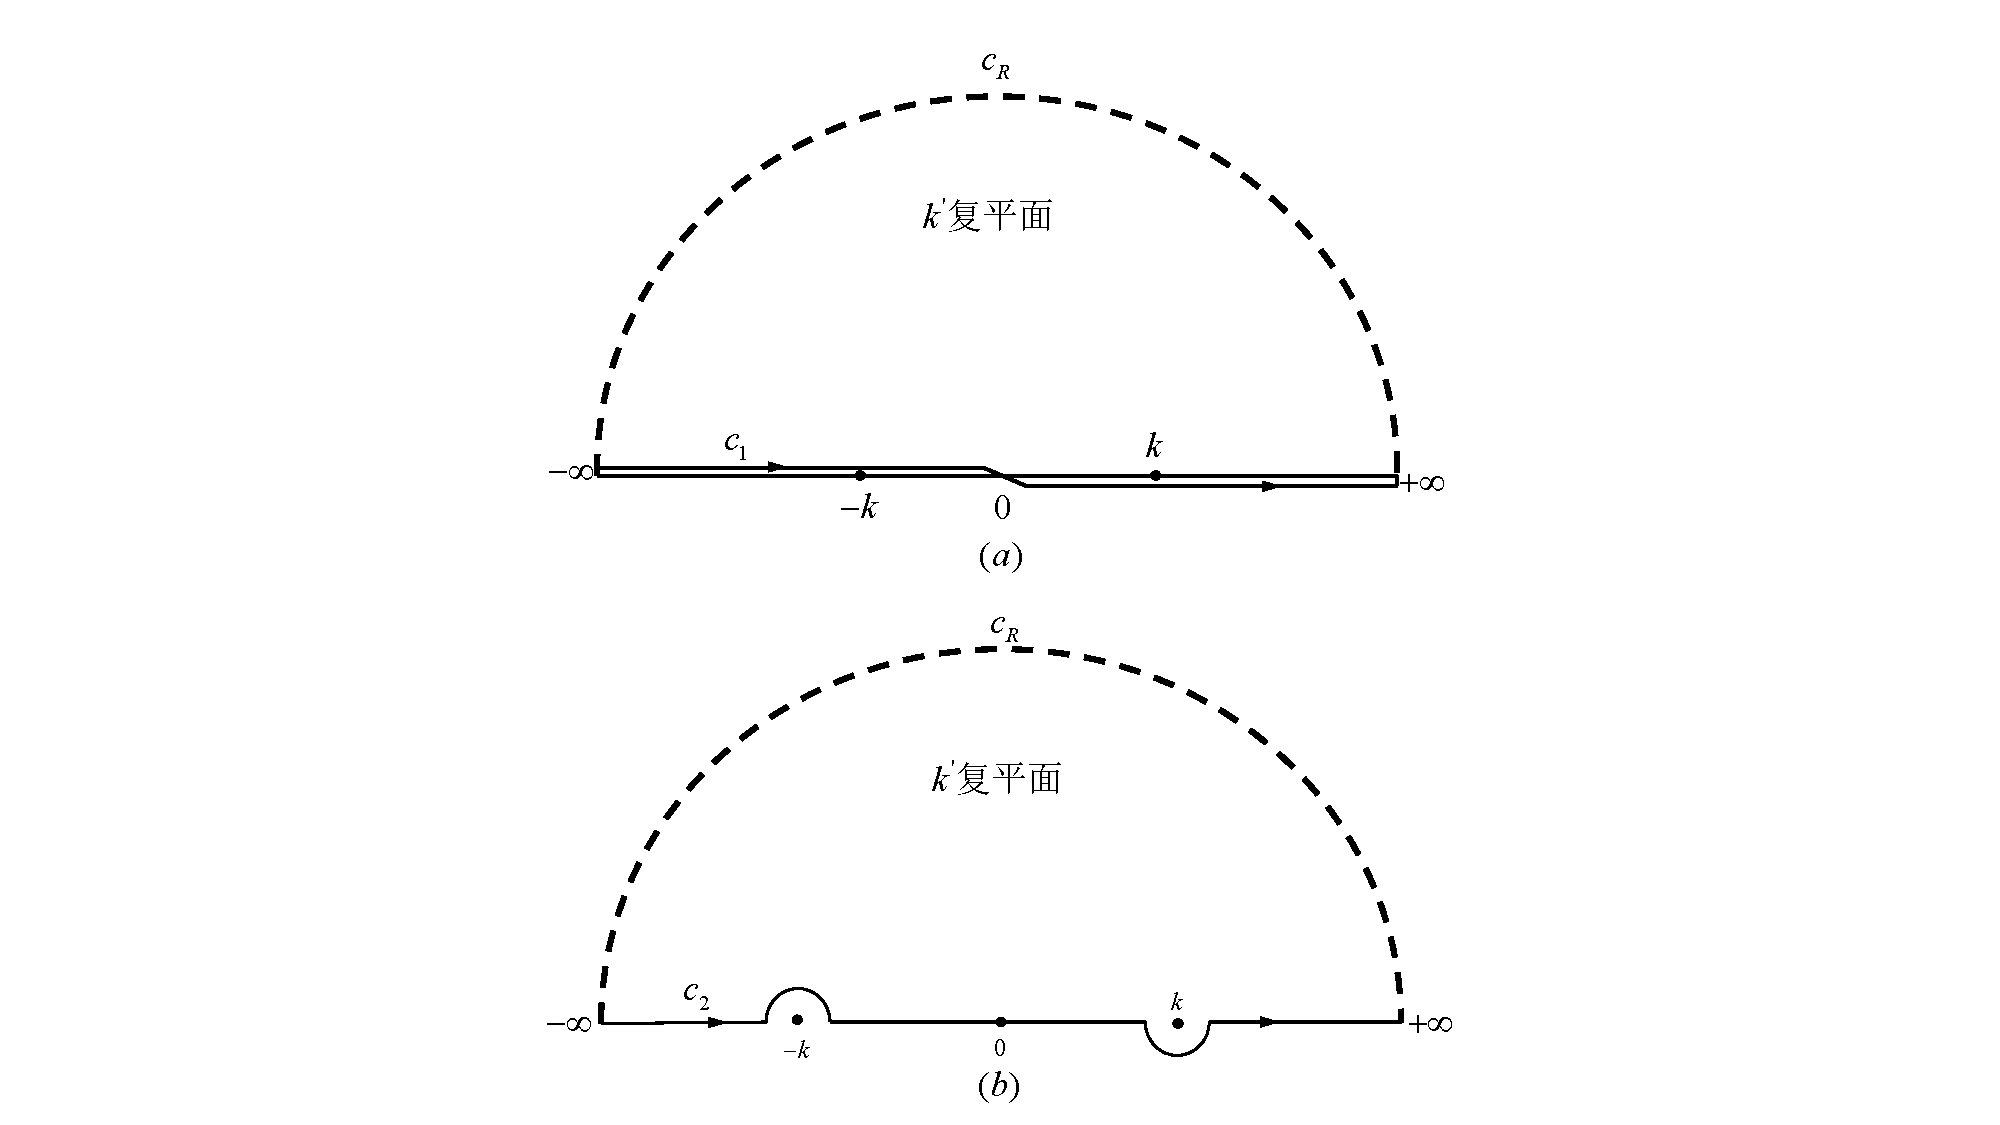
\includegraphics[width=5.5cm,clip]{QM file/figure/8-5}
	\caption{}\label{fig.8-5}
\end{figure}
上式可用$\boldsymbol{k}^{\prime}$复平面上围道积分法算出.但$k^{\prime}=\pm k$是被积函数的一级极点,为了确保$G(\boldsymbol{r},\boldsymbol{r}^{\prime})$中只有出射波,[这样才能符合边界条件\eqref{eq84.7}式]在$\boldsymbol{k}^{\prime}$复平面的左半,积分路线应取实轴上岸,在$\boldsymbol{k}^{\prime}$复平面的右半,积分路线应取实轴下岸,如图\ref{fig.8-5}(a)所示,亦即\eqref{eq84.20}式中积分路线规定为
\begin{empheq}{equation}\label{eq84.21}
	\int_{-\infty}^{\infty}\cdots dk^{\prime}\Rightarrow\int_{c_{1}}\cdots dk^{\prime}
\end{empheq}
这个规定等价于\eqref{eq84.20}式中$k$换成$k+i\varepsilon$($\varepsilon$为无限小正实数) ,或等价于沿图\ref{fig.8-5}(b)中路径$c_{2}$的积分.注意,图\ref{fig.8-5}中沿大圆弧$c_{R}$的积分为0.按照复平面围道积分的残数定理,容易算出
\begin{empheq}{equation}\label{eq84.22}
	\boxed{G(\boldsymbol{r},\boldsymbol{r}^{\prime})=-\frac{\exp(ik|\boldsymbol{r}-\boldsymbol{r}^{\prime}|)}{4\pi|\boldsymbol{r}-\boldsymbol{r}^{\prime}|}}
\end{empheq}
这正是符合散射波性质的出射波形式格林函数.反之,如取积分路径为图\ref{fig.8-5}中(a)实轴下岸及(b)实轴上岸,[相当于\eqref{eq84.20}式中$k$换成$k+i\varepsilon$]则给出
\begin{empheq}{equation*}
	G(\boldsymbol{r},\boldsymbol{r}^{\prime})=-\frac{\exp(ik|\boldsymbol{r}-\boldsymbol{r}^{\prime}|)}{4\pi|\boldsymbol{r}-\boldsymbol{r}^{\prime}|}
\end{empheq}
就不符合散射波的性质,不能采用.


{\heiti 3. 玻恩近似}

将格林函数\eqref{eq84.22}式代入\eqref{eq84.16}式,得到$\varPsi^{(1)}$的明显表示式
\eqlong
\begin{empheq}{equation}\label{eq84.23}
	\varPsi^{(1)}=-\frac{\mu}{2\pi\hbar^{2}}\int\frac{\exp(ik|\boldsymbol{r}-\boldsymbol{r}^{\prime}|)}{|\boldsymbol{r}-\boldsymbol{r}^{\prime}|}V(\boldsymbol{r}^{\prime})\varPsi^{(0)}(\boldsymbol{r}^{\prime})d^{3}\boldsymbol{r}^{\prime}
\end{empheq}\eqnormal
为了得到散射振幅的一级近似$f^{(1)}$,只需要求出$r\rightarrow\infty$处$\varPsi^{(1)}$的函数形式,由于$r\gg r^{\prime}$,可以取下列近似(参看图\ref{fig.8-6}):
\begin{empheq}{equation}\label{eq84.24}
	k|\boldsymbol{r}-\boldsymbol{r}^{\prime}|\approx k\bigg(r-\frac{\boldsymbol{r}^{\prime}\cdot\boldsymbol{r}}{r}\bigg)=kr-\boldsymbol{k}\cdot\boldsymbol{r}^{\prime}
\end{empheq}

\begin{figure}[!h]
	\centering
	\small
	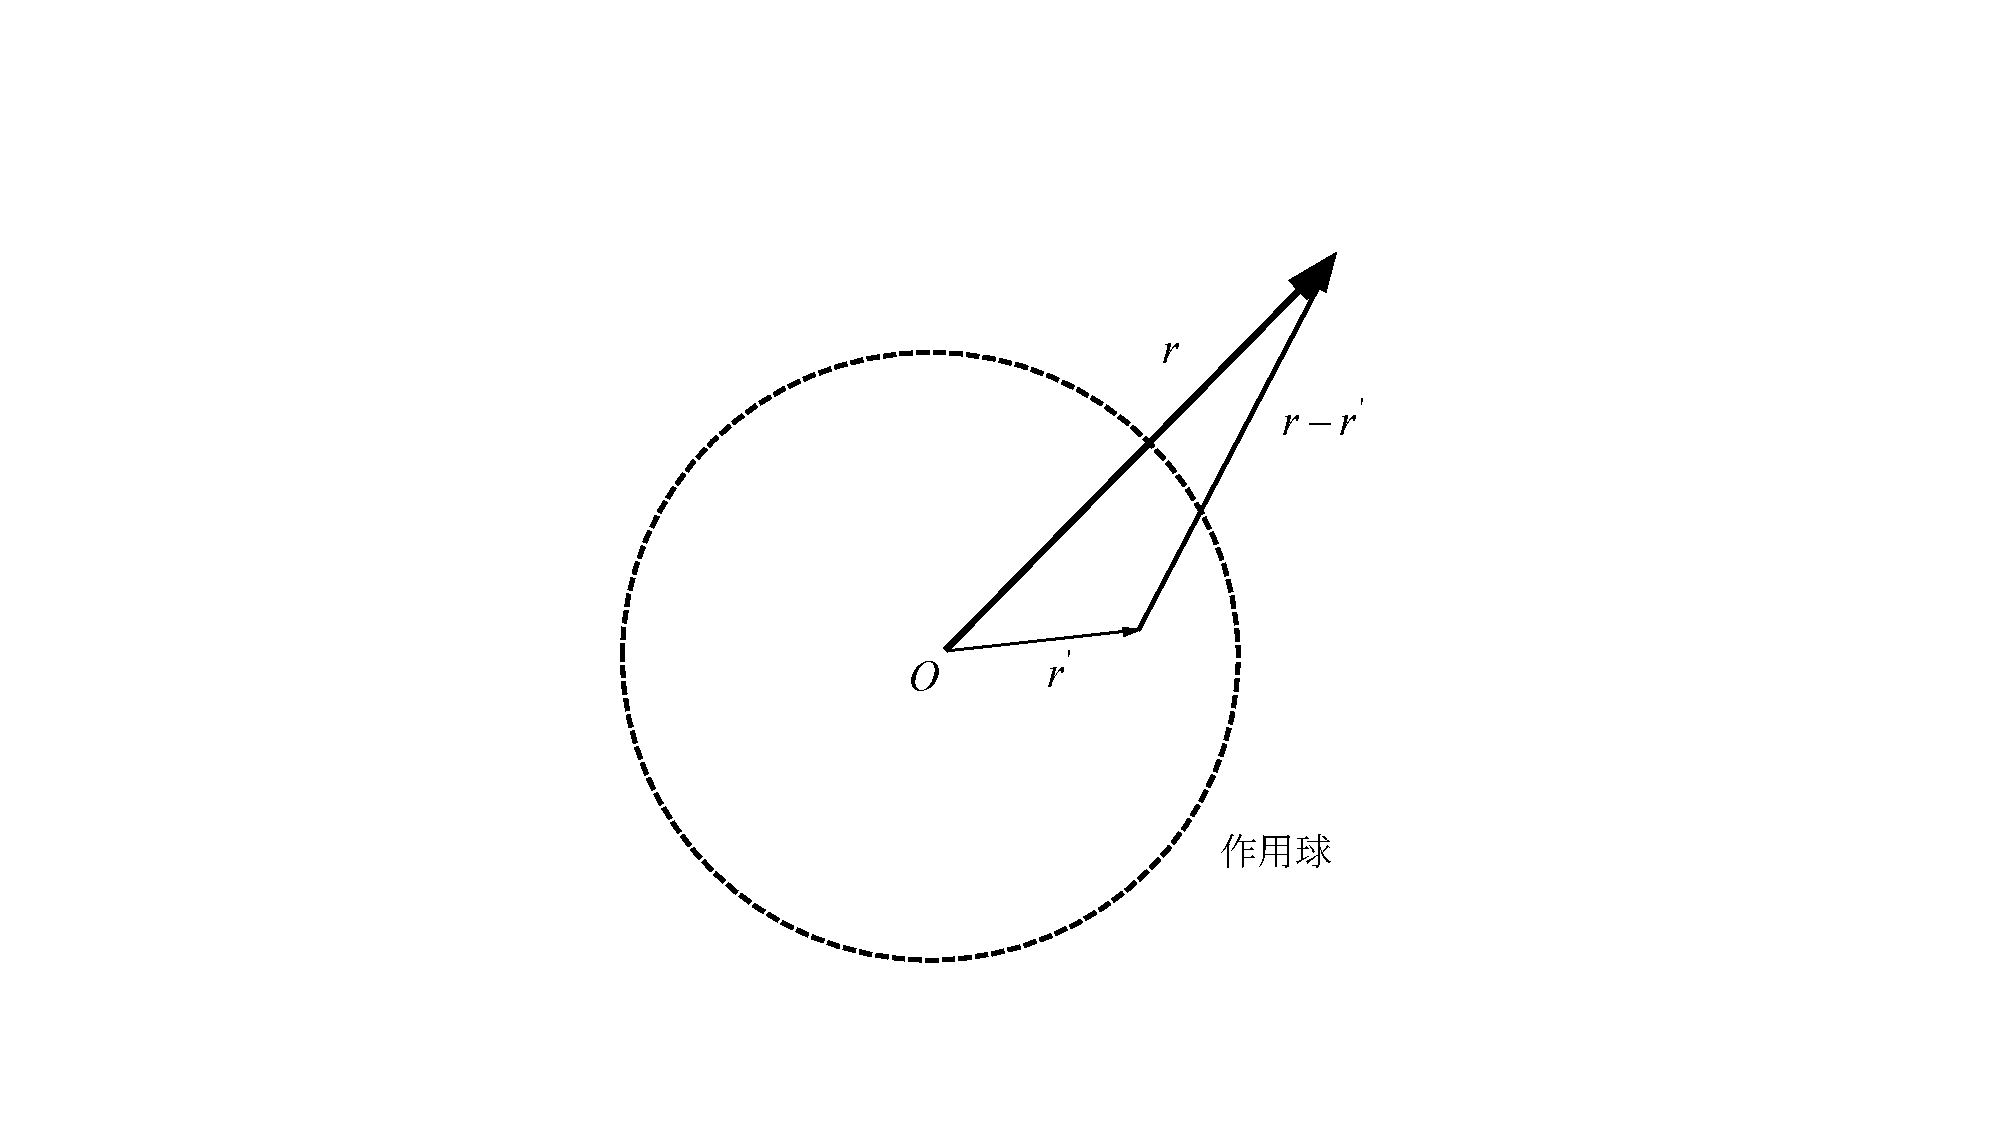
\includegraphics[width=5cm,clip]{QM file/figure/8-6}
	\caption{}\label{fig.8-6}
\end{figure}
$\boldsymbol{k}$为出射波波矢量,其方向即$\boldsymbol{r}$的方向,$\boldsymbol{k}=k\frac{\boldsymbol{r}}{r}$.对于\eqref{eq84.5}式及\eqref{eq84.23}式中的入射波波函数,可表示成
\begin{empheq}{align*}
	\varPsi^{(0)(\boldsymbol{r})}&=e^{ikz}=e^{i\boldsymbol{k}_{0}\cdot\boldsymbol{r}}	\tag{$8.4.5^{\prime}$}\label{eq84.5'}\\
	\varPsi^{(0)(\boldsymbol{r}^{\prime})}&=e^{ikz^{\prime}}=e^{i\boldsymbol{k}_{0}\cdot\boldsymbol{r}^{\prime}}	\tag{$8.4.5^{\prime\prime}$}\label{eq84.5''}\\
\end{empheq}
\noindent$k_{0}$为入射波波矢量,其方向即$z$轴及$z^{\prime}$轴方向.将\eqref{eq84.24}式及\eqref{eq84.5''}式代入\eqref{eq84.23}式,并取\eqref{eq84.23}式中分母$|\boldsymbol{r}-\boldsymbol{r}^{\prime}|$$\approx r$,得到
\eqlong
\begin{empheq}{align}\label{eq84.25}
	\varPsi^{(1)}(\boldsymbol{r}) &\approx-\frac{\mu}{2\pi\hbar^{2}}\frac{e^{ikr}}{r}\int V(\boldsymbol{r}^{\prime})\exp[i(\boldsymbol{k_{0}}-\boldsymbol{k})\cdot\boldsymbol{r}^{\prime}]d^{3}\boldsymbol{r}^{\prime}	\nonumber\\
	&=-\frac{\mu}{2\pi\hbar^{2}}V(\boldsymbol{k},\boldsymbol{k_{0}})\frac{e^{ikr}}{r}
\end{empheq}
\eqnormal
其中
\begin{empheq}{equation}\label{eq84.26}
	V(\boldsymbol{k},\boldsymbol{k_{0}})=\int V(\boldsymbol{r}^{\prime})\exp[i(\boldsymbol{k_{0}}-\boldsymbol{k})\cdot\boldsymbol{r}^{\prime}]d^{3}\boldsymbol{r}^{\prime}
\end{empheq}
比较\eqref{eq84.7}式及\eqref{eq84.25}式,即得散射振幅的一级近似:
\begin{empheq}{equation}\label{eq84.27}
	\boxed{f^{(1)}(\theta,\varphi)=-\frac{\mu}{2\pi\hbar^{2}}V(\boldsymbol{k},\boldsymbol{k_{0}})	}
\end{empheq}
$\boldsymbol{k}$的方向即$(\theta,\varphi)$方向.$(\hbar\boldsymbol{k}-\hbar\boldsymbol{k_{0}})$是散射过程中粒子的动量变化,常被称为“动量转移”,记为$\hbar q$,即
\begin{empheq}{equation}\label{eq84.28}
	\boxed{\boldsymbol{q}=\boldsymbol{k}-\boldsymbol{k_{0}},\quad q=2k\sin\frac{\theta}{2}	}
\end{empheq}

\begin{wrapfigure}[9]{r}{8em}
	\centering
	\small
	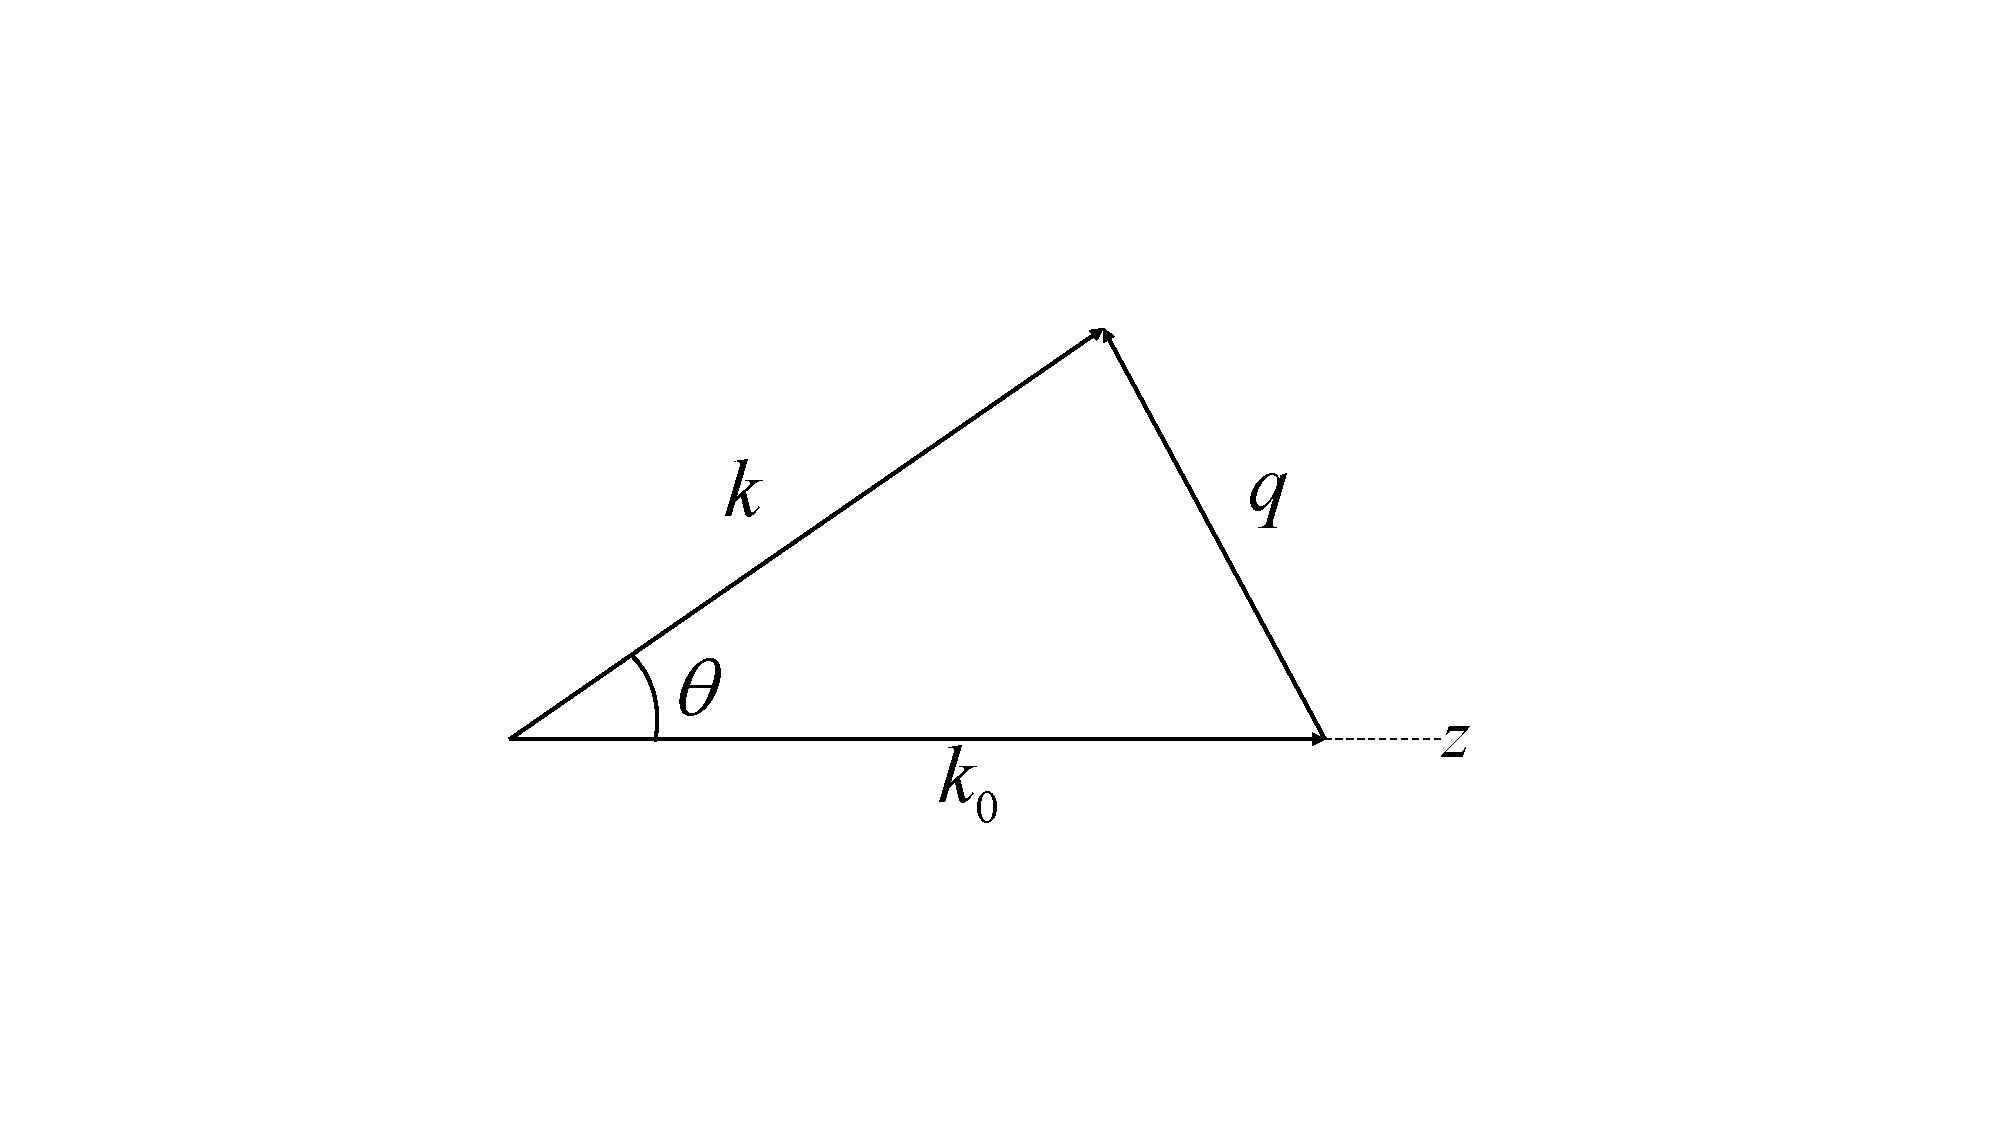
\includegraphics[width=3cm,clip]{QM file/figure/8-7}
	\caption{}\label{fig.8-7}
\end{wrapfigure}
如图\ref{fig.8-7}所示,用$\boldsymbol{q}$代替$(\boldsymbol{k}-\boldsymbol{k_{0}})$,\eqref{eq84.26}式可以写成
\eqindent{4}
\begin{empheq}{equation*}\label{eq84.26'}
	V(\boldsymbol{k},\boldsymbol{k_{0}})=\int V(\boldsymbol{r}^{\prime})	e^{-i\boldsymbol{q}\cdot\boldsymbol{r}^{\prime}}	d^{3}\boldsymbol{r}^{\prime}	\tag{$8.4.26^{\prime}$}
\end{empheq}\eqnormal

如果是中心力散射,$V(\boldsymbol{r}^{\prime})=V(r^{\prime})$,\eqref{eq84.26'}式中角部积分与$V$无关,可以直接算出,如下.$\boldsymbol{r}^{\prime}$空间用球坐标,并以$-\boldsymbol{q}$方向作为极轴方向,则$$-\boldsymbol{q}\cdot\boldsymbol{r}^{\prime}=qr^{\prime}\cos\theta^{\prime},\quad d^{3}\boldsymbol{r}^{\prime}=r^{\prime2}dr^{\prime}\sin\theta^{\prime}d\theta^{\prime}d\varphi^{\prime}$$
\eqlong
\begin{empheq}{align}\label{eq84.29}
	\int e^{-i\boldsymbol{q}\cdot\boldsymbol{r}^{\prime}}\sin\theta^{\prime}d\theta^{\prime}d\varphi&=2\pi\int_{0}^{\pi}e^{iqr^{\prime}\cos\theta^{\prime}}\sin\theta^{\prime}d\theta^{\prime}	\nonumber\\
	&=\frac{4\pi}{qr^{\prime}}\sin qr^{\prime}
\end{empheq}\eqnormal
因此
\begin{empheq}{equation}\label{eq84.30}
	V(\boldsymbol{k},\boldsymbol{k_{0}})=4\pi\int_{0}^{\infty}V(r^{\prime})\frac{\sin qr^{\prime}}{qr^{\prime}}r^{\prime2}dr^{\prime}
\end{empheq}
\begin{empheq}{equation}\label{eq84.31}
	\boxed{f^{(1)}(\theta)=-\frac{2\mu}{\hbar^{2}}\int_{0}^{\infty}V(r^{\prime})\frac{\sin qr^{\prime}}{qr^{\prime}}r^{\prime2}dr^{\prime}	}
\end{empheq}
由于$q=2k\sin\bigg(\frac{\theta}{2}\bigg)$,所以$f^{(1)}$是散射角$\theta$的函数.

如果略去二级修正,则微分散射截面为
\begin{empheq}{equation}\label{eq84.32}
	\sigma(\theta,\varphi)\approx|f^{(1)}|^{2}=\frac{\mu^{4}}{4\pi^{2}\hbar^{4}}|V(\boldsymbol{k},\boldsymbol{k_{0}})|^{2}
\end{empheq}
对于中心力场散射,微分散射截面仅为$\theta$的函数,
\begin{empheq}{equation}\label{eq84.33}
	\sigma(\theta)\approx\frac{4\mu^{2}}{\hbar^{4}}\bigg[\int_{0}^{\infty}V(r^{\prime})\frac{\sin qr^{\prime}}{qr^{\prime}}r^{\prime2}dr^{\prime}\bigg]^{2}
\end{empheq}
以上结果[主要指\eqref{eq84.25}、\eqref{eq84.27}、\eqref{eq84.32}式]通常称为玻恩(M.Born)近似.

{\heiti 4. 玻恩近似的适用条件}

\eqref{eq84.2}式或\eqref{eq84.10}式的严格解应该写成
\begin{empheq}{align*}\label{eq84.10'}
	\varPsi_{s}(\boldsymbol{r}) &=(\nabla^{2}+k^{2})^{-1}\frac{2\mu}{\hbar^{2}}V(\boldsymbol{r})\varPsi(\boldsymbol{r})	\\
	&=\frac{2\mu}{\hbar^{2}}\int G(\boldsymbol{r},\boldsymbol{r}^{\prime})V(\boldsymbol{r}^{\prime})\varPsi(\boldsymbol{r}^{\prime})d^{3}\boldsymbol{r}^{\prime}
	\tag{$8.4.10^{\prime}$}
\end{empheq}
由于$\varPsi=\varPsi^{(0)}+\varPsi_{s}$,上式为积分方程\eqref{eq84.16}式是上式的一级近似解,相当于在右端的积分中以$\varPsi^{(0)}$代替$\varPsi$.由此可知\eqref{eq84.16}式和\eqref{eq84.23}式的适用条件是在散射区内$(r\sim r^{\prime})|\varPsi^{(1)}(\boldsymbol{r})|\ll|\varPsi^{(0)}(\boldsymbol{r})|$,亦即
\begin{empheq}{equation}\label{eq84.34}
	|\varPsi^{(1)}(\boldsymbol{r})|\ll1\quad (r\sim r^{\prime})
\end{empheq}
通常,作用势$V(\boldsymbol{r}^{\prime})$总是存在一定的有效范围(作用球,半径$a$),在作用球内,$V$变化平缓,在作用球外,$V$迅速减弱.作为数量级估算,\eqref{eq84.23}式中$V(\boldsymbol{r}^{\prime})$不妨用平均值$V_{0}$来代替,而积分在作用球内进行.这样做相当于采用球形势垒(阱)模型.通常,在力心附近$(r\sim 0)$散射作用较强,所以\eqref{eq84.34}式可取$r=0$进行估算,即适用条件取为
\eqlong
\begin{empheq}{equation}\label{eq84.35}
	|\varPsi^{(1)}(0)|\approx\frac{\mu|V_{0}|}{2\pi\hbar^{2}}\bigg|\int\frac{d^{3}\boldsymbol{r}^{\prime}}{r^{\prime}}\exp[ikr^{\prime}+i\boldsymbol{k_{0}}\cdot\boldsymbol{r}^{\prime}]\bigg|\ll1
\end{empheq}\eqnormal
其中$\exp(i\boldsymbol{k_{0}}\cdot\boldsymbol{r}^{\prime})=\exp(ikz^{\prime})=\varPsi^{(0)}(\boldsymbol{r}^{\prime})$.

对于低能散射,$ka\ll 1$,\eqref{eq84.35}式中指数函数近似等于1,而
\begin{empheq}{equation*}
	\int\frac{d^{3}\boldsymbol{r}^{\prime}}{r^{\prime}}\approx4\pi\int_{0}^{a}r^{\prime}d^{\prime}=2\pi a^{2}
\end{empheq}
所以适用条件为
\begin{empheq}{equation}\label{eq84.36}
	|\varPsi^{(1)}(0)|\approx \mu|V_{0}|\frac{a^{2}}{\hbar^{2}}\ll1
\end{empheq}
要满足此式,势垒(阱)必须充分弱($|V_{0}|$小)而窄($a$小).

对于高能散射,$ka\gg1$,\eqref{eq84.35}式中指数函数在$0<r^{\prime}<a$范围内将多次振荡,必须作出较精确的估算,采用球坐标$(r^{\prime},\theta^{\prime},\varphi^{\prime})$,将\eqref{eq84.35}式中角部积分算出[参看\eqref{eq84.29}式],
\begin{empheq}{equation*}
	\int e^{i\boldsymbol{k}_{0}\cdot\boldsymbol{r}}\sin\theta^{\prime}d\varphi^{\prime}=4\pi\frac{\sin kr^{\prime}}{kr^{\prime}}
\end{empheq}
所以
\eqlong
\begin{empheq}{align}\label{eq84.37}
	&\int\frac{d^{3}\boldsymbol{r}^{\prime}}{r^{\prime}}\exp(ikr^{\prime}+i\boldsymbol{k_{0}}\cdot\boldsymbol{r}^{\prime})=\frac{4\pi}{k}\int_{0}^{a}\sin kr^{\prime}e^{ikr^{\prime}}dr^{\prime}	\nonumber\\
	=&\frac{4\pi}{k^{2}}\int_{0}^{ak}\sin xe^{ix}dx=\frac{4\pi}{k^{2}}\bigg[\frac{i}{2}ak+\frac{1}{4}(1-e^{2iak})\bigg]	\nonumber\\
	=&\frac{4\pi}{k^{2}}\cdot\frac{i}{2}ak=2i\pi\frac{a}{k}
\end{empheq}\eqnormal
代入\eqref{eq84.35},即得适用条件为
\begin{empheq}{equation}\label{eq84.38}
	|\varPsi^{(1)}(0)|\approx \mu|V_{0}|\frac{a}{\hbar^{2}k}\ll1
\end{empheq}
即
\begin{empheq}{equation*}\label{eq84.38'}
	\mu|V_{0}|\frac{a^{2}}{\hbar^{2}}\ll ak\quad\text{或}\quad 2|V_{0}|ak\ll\frac{\hbar^{2}k^{2}}{2\mu}=E
	\tag{$8.4.38^{\prime}$}
\end{empheq}
显然,入射粒子的动能$\bigg(E=\frac{\hbar^{2}k^{2}}{2\mu}\bigg)$越大,条件\eqref{eq84.38'}越易满足.注意,对于一定的势场$(V_{0},a)$,玻恩近似是否适用于低能散射,即\eqref{eq84.36}式是否成立,是由势场本身决定的;而对于高能散射,只要入射能量足够大,总能使\eqref{eq84.38}式成立,即玻恩近似可以适用.另外,比较\eqref{eq84.36}及\eqref{eq84.38}式,可知$|\varPsi^{(1)}(0)|^{2}$之值在高能散射时约为低能散射时的$(ak)^{-2}$倍,由此可以估计,两种情况下总散射截面大致也相差$(ak)^{-2}$倍.

顺便讨论一下中心力散射的玻恩近似\eqref{eq84.31}、\eqref{eq84.33}式.在低能散射条件$(ka\ll1)$下,对于任何散射$\theta$,均有
\begin{empheq}{align*}
	qr^{\prime}=2kr^{\prime}&\sin\bigg(\frac{\theta}{2}\bigg)<2ka\ll1	\\
	&\frac{\sin qr^{\prime}}{qr^{\prime}}\approx 1
\end{empheq}
\eqref{eq84.31}式给出
\begin{empheq}{equation}\label{eq84.39}
	f^{(1)}\approx -\frac{2\mu}{\hbar^{2}}\int_{0}^{\infty}V(r^{\prime})r^{\prime2}dr^{\prime}
\end{empheq}
$f(\theta)\approx f^{(1)}$与$\theta$无关,这结果相当于分波法中低能s波$(l=0)$散射.例如对于球形势阱$(V=-V_{0},r<a)$,上式给出
\begin{empheq}{align}\label{eq84.40}
	&f(\theta)\approx f^{(1)}\approx\frac{2\mu V_{0}a^{3}}{3\hbar^{2}}		\nonumber\\
	\sigma_{\text{总}}&\approx 4\pi|f|^{2}=\frac{16\pi}{9}\bigg(\frac{\mu V_{0}a^{3}}{\hbar^{2}}\bigg)^{2}
\end{empheq}
这正是\eqref{eq83.21}式.$\S$\ref{sec:08.03}例题中提到的条件$ka\ll1$,正是玻恩近似的适用条件,即本节\eqref{eq84.36}式注意,由于条件\eqref{eq84.36}式,$\sigma_{\text{总}}\ll\pi a^{2}$.

仍以球形势阱(或势垒,强度$V_{0}$,半径$a$)为例,对高能散射作定性讨论.\eqref{eq84.31}式中以$\pm V_{0}$代替$V(r^{\prime})$后,积分可以简单算出,
\eqlong
\begin{empheq}{align}\label{eq84.41}
	&\int_{0}^{a}\frac{\sin qr^{\prime}}{qr^{\prime}}r^{\prime2}dr^{\prime}=q^{-3}\int_{0}^{aq}x\sin xdx		\nonumber\\
	=&a^{3}(\sin aq-aq\cos a)(aq)^{-3}=a^{3}F(aq)
\end{empheq}\eqnormal
其中$a_{q}=2ak\sin\bigg(\frac{\theta}{2}\bigg)$.当$aq<\pi$,$F(aq)$随$aq$之增大而徐缓减小,$(aq=0.1,F=0.33;aq=1,F=0.30;aq=2,F=0.22;aq=\pi,F=0,10)$当$aq>\pi$,$|F(aq)|$迅速减小$(aq=4.49,F\sim0;aq=5,F=-\num{0.019};aq=2\pi,F=-\num{0.025};aq=3\pi,F=\num{0.011})$.因此,仅当$\theta<\pi/ak(aq\sim ak\theta<\pi)$,$f(\theta)$及$\sigma(\theta)$才有显著的值(但对$\theta$的变化不敏感).这就是说,在玻恩近似成立的前提下,大部分散射粒子的散射角$\theta<\frac{\pi}{ak}$.相应的$f(\theta)$约为
\begin{empheq}{align}\label{eq84.42}
	|f(\theta)|\approx \frac{2\mu V_{0}a^{3}}{\hbar^{2}}F(aq)\lesssim\frac{2\mu V_{0}a^{3}}{3\hbar^{2}}
\end{empheq}
$\bigg(F\lesssim\frac{1}{3}\bigg)$而总散射截面约为
\begin{empheq}{align}\label{eq84.43}
	\sigma_{\text{总}} &=\int|f(\theta)|^{2}\sin\theta d\theta d\varphi	\nonumber\\
	&\lesssim\bigg(\frac{2\mu V_{0}a^{3}}{3\hbar^{2}}\bigg)^{2}2\pi\int_{0}^{\frac{\pi}{ak}}\sin\theta d\theta	\nonumber\\
	&\sim \bigg(\frac{2\mu V_{0}a^{3}}{3\hbar^{2}}\bigg)\frac{\pi^{3}}{(ak)^{2}}\propto\frac{1}{k^{2}}\propto\frac{1}{E}
\end{empheq}
按量级说,大致是低能$\sigma_{\text{总}}$的$(ak)^{-2}$倍.注意,由于条件\eqref{eq84.38'}式,易见$\sigma_{\text{总}}\ll4\pi a^{2}$,这意味着散射是微弱的.而且,$\sigma_{\text{总}}$大体上与$E$成反比.
\pskip

\example 质量为$\mu$的粒子束以动量$\hbar k$入射,遇中心力场
\begin{empheq}{equation}\label{eq84.44}
	V(r)=\frac{B}{r}e^{-r/a}\quad (a>0)
\end{empheq}
求散射截面的玻恩近似(一级近似).并讨论$ka\gg1,ka\ll1,a\rightarrow\infty$等极限情形.

\solution 在玻恩近似下,散射振幅由\eqref{eq84.31}式表示,即
\begin{empheq}{align}\label{eq84.45}
	f(\theta) &=-\frac{2\mu B}{\hbar^{2}q}\int_{0}^{\infty}\sin qre^{-r/a}dr	\nonumber\\
	&=-\frac{2\mu B}{\hbar^{2}q}\cdot\frac{qa^{2}}{1+q^{2}a^{2}}	\nonumber\\
	&=-\frac{2\mu Ba^{2}}{\hbar^{2}}\cdot\frac{1}
	{1+4a^{2}k^{2}\sin^{2}\bigg(\frac{\theta}{2}\bigg)}
\end{empheq}
微分散射截面及总散射截面为
\begin{empheq}{equation*}
	\sigma(\theta)=|f(\theta)|^{2},\quad \sigma_{\text{总}}=2\pi\int_{0}^{\pi}\sigma(\theta)\sin\theta d\theta
\end{empheq}
可以算出
\begin{empheq}{equation}\label{eq84.46}
	\sigma_{\text{总}}=\frac{16\pi\mu^{2}B^{2}a^{4}}{\hbar^{2}(1+4a^{2}k^{2})}
\end{empheq}
由\eqref{eq84.44}式表示的作用势,可以用于许多问题.反映核子-核子作用力的“汤川(Yukawa)势”正是这种形式,$a$代表力程$(a\sim 2\si{fm})$,$B/a$代表平均作用强度(约$20\sim30\si{MeV}$).带电粒子被原子散射,\eqref{eq84.44}式可以近似表示“屏蔽库仑势”,因子$e^{-r/a}$代表原子的电子壳层对于核电荷的屏蔽效应($a\sim$原子半径).纯库仑势$V\propto\frac{1}{r}$,相当于$a\rightarrow\infty$这种极端的情形.

高能散射,$ka\gg1$,在\eqref{eq84.45}式中只要$\theta$不太小,能使$qa\gg1$,则
\begin{empheq}{align}
	f(\theta) &\approx-\frac{\mu B}{2\hbar^{2}k^{2}\sin^{2}\bigg(\frac{\theta}{2}\bigg)}				\label{eq84.47}\\
	\sigma(\theta)
	&\approx\frac{\mu^{2}B^{2}}{4\hbar^{4}k^{4}\sin^{4}\bigg(\frac{\theta}{2}\bigg)}\nonumber\\
	&=\frac{B^{2}}{16E^{2}\sin^{4}\bigg(\frac{\theta}{2}\bigg)} \label{eq84.48}
\end{empheq}
这结果相当于$a\rightarrow\infty$的情况,即纯库仑势散射.但是,对于纯库仑势,上式也适用于很小的散射角,因此$\sigma_{\text{总}}\rightarrow\infty$.而对于力程$\theta$有限的情况,\eqref{eq84.48}式只适用于$qa\gg1$,即$\theta\gg\frac{1}{ka}$.当$\theta\rightarrow0$,\eqref{eq84.45}式给出$f(0)=-\frac{2\mu Ba^{2}}{\hbar^{2}}$,为有限值.\eqref{eq84.46}式在$ka\gg1$条件下给出
\begin{empheq}{equation}\label{eq84.49}
	\sigma_{\text{总}}\overset{ka\gg1}{\longrightarrow}4\pi\frac{\mu^{2}B^{2}a^{2}}{\hbar^{4}k^{2}}\propto\frac{1}{E}
\end{empheq}
这结果与\eqref{eq84.43}式大致符合$(B\sim V_{0}a)$.

低能散射,$ka\ll1$,对任何散射角$\theta$,均有$qa\gg1$,\eqref{eq84.45}式给出
\begin{empheq}{equation}\label{eq84.50}
	f(\theta)\approx -\frac{2\mu Ba^{2}}{\hbar^{2}},\quad \sigma(\theta)\approx \frac{4\mu^{2}B^{2}a^{4}}{\hbar^{4}}
\end{empheq}
$\sigma(\theta)$与$\theta$无关,这是低能散射的特点.在$ka\ll1$条件下,玻恩近似的适用条件为
\eqlong
\begin{empheq}{equation}\label{eq84.51}
	|\varPsi_{s}(0)|\approx\frac{2\mu}{\hbar^{2}}\cdot\frac{1}{4\pi}\bigg|\int V(\boldsymbol{r})\frac{d^{3}\boldsymbol{r}}{r}\bigg|=\frac{2\mu a}{\hbar^{2}}|B|\ll1
\end{empheq}\eqnormal
所以
\begin{empheq}{equation*}
	\sigma_{\text{总}}=4\pi\sigma(\theta)=4\pi a^{2}\bigg(\frac{2\mu Ba}{\hbar^{2}}\bigg)^{2}\ll 4\pi a^{2}
\end{empheq}

在许多问题中,条件\eqref{eq84.51}往往不成立.例如核子-核子散射,$a\sim2\si{fm},\frac{B}{a}\sim30\si{MeV},2\mu c^{2}\sim938\si{MeV}$,则
\eqlong
\begin{empheq}{equation*}
	\frac{2\mu Ba}{\hbar^{2}}=\frac{2\mu c^{2}Ba}{(\hbar c)^{2}}\sim\frac{938\times30\times4(\si{MeV}\cdot\si{fm})^{2}}{(200\si{MeV}\cdot\si{fm})^{2}}\sim 2.8
\end{empheq}\eqnormal
所以核子-核子低能散射一般不能用玻恩近似处理,而必须用分波法.

